\section{F2LLM-v2}

\begin{figure}[t]
    \centering
    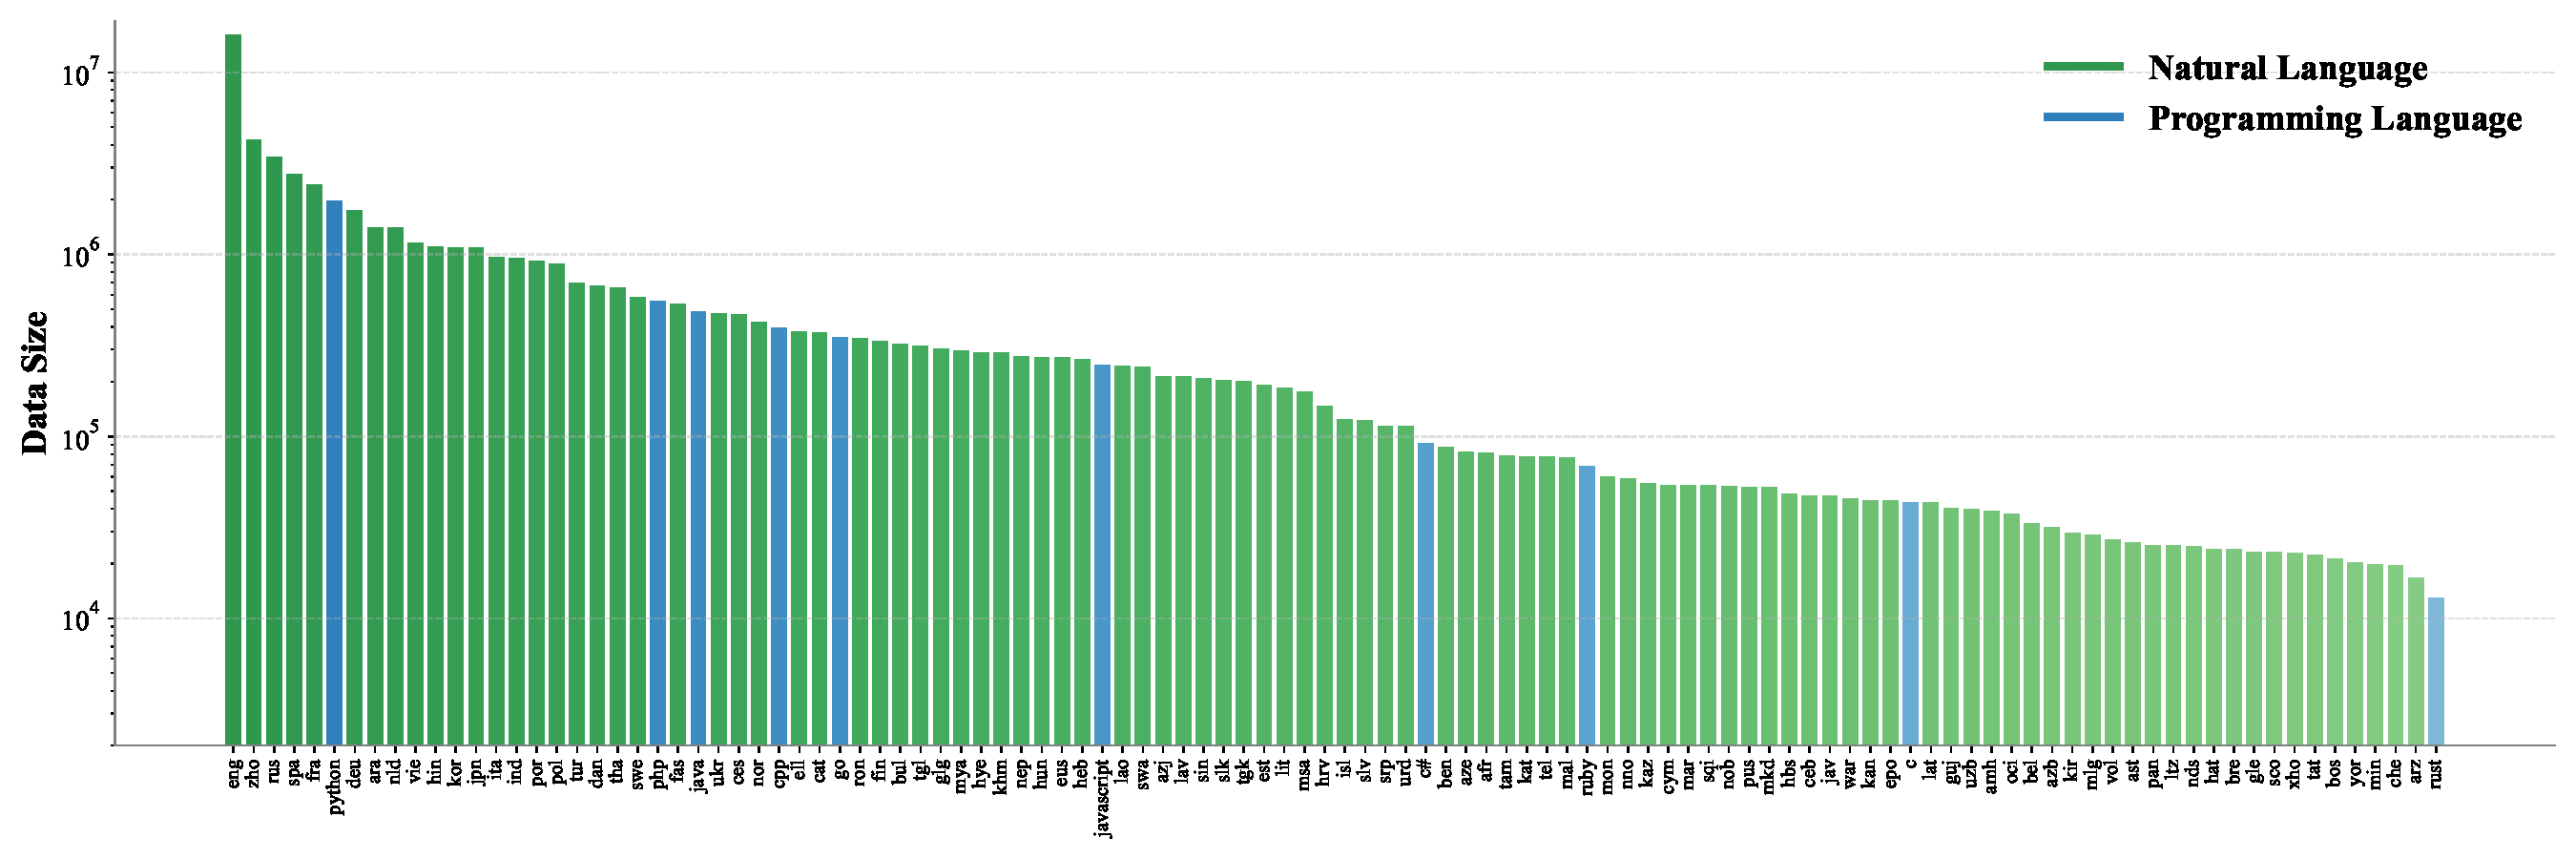
\includegraphics[width=1.0\linewidth]{figures/language_distribution.pdf}
    \caption{Top-100 natural languages and top-10 programming languages in our training data.}
    \label{fig:language-distribution}
\end{figure}

\subsection{Training Data}

\begin{wrapfigure}{r}{0.5\linewidth}
    \centering
    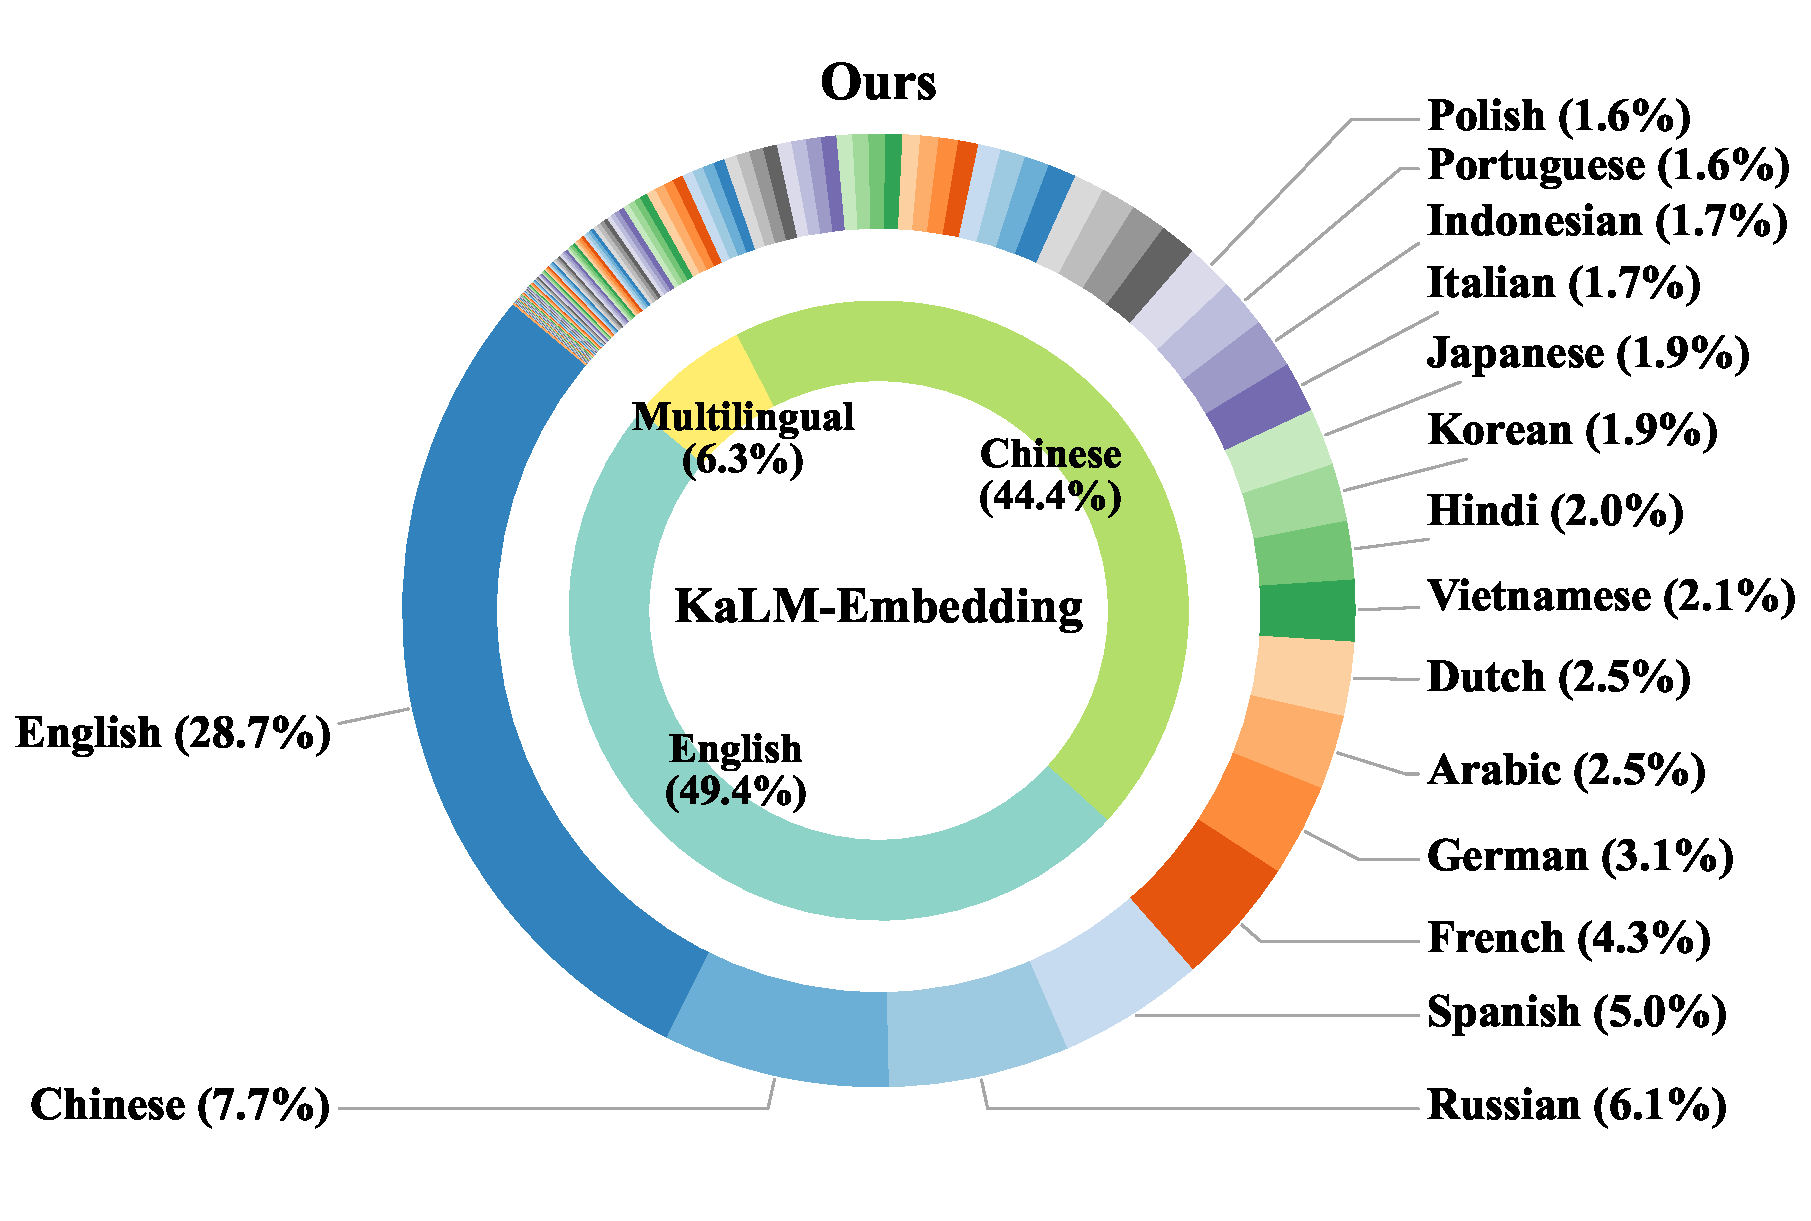
\includegraphics[width=1\linewidth]{figures/language_percentage.pdf}
    \caption{Comparison between the language distribution of our training data (outer circle) and KaLM-Embedding (inner circle). KaLM-Embedding's data is only annotated with three labels, while ours are annotated with specific languages.}
    \label{fig:language-comparison}
\end{wrapfigure}

A cornerstone of F2LLM-v2 is the compilation of a vast and diverse training corpus designed to foster both linguistic inclusivity and broad task competency. We aggregate data from 157 publicly available sources, creating a collection of 60 million training samples that span 282 natural languages (as identified by ISO-639-3 codes) and over 40 programming languages. Crucially, our data curation process is driven by real-world data availability rather than optimizing for specific benchmarks. For instance, our dataset contains substantial data for Spanish, Arabic, Italian, Indonesian, and Portuguese (Figure~\ref{fig:language-distribution}), despite these languages lacking dedicated benchmarks in MTEB. This approach, which also includes a long tail of low-resource languages and a significant volume of code, aims to build a model with truly global utility and stands in direct contrast to recent open-source datasets such as the one released by KaLM-Embedding~\citep{2025KaLM-Embedding-V2}, which is heavily skewed towards English and Chinese (Figure~\ref{fig:language-comparison}). We provide a more comprehensive linguistic breakdown of our dataset in Appendix~\ref{appendix:data}.


\begin{figure}
    \centering
    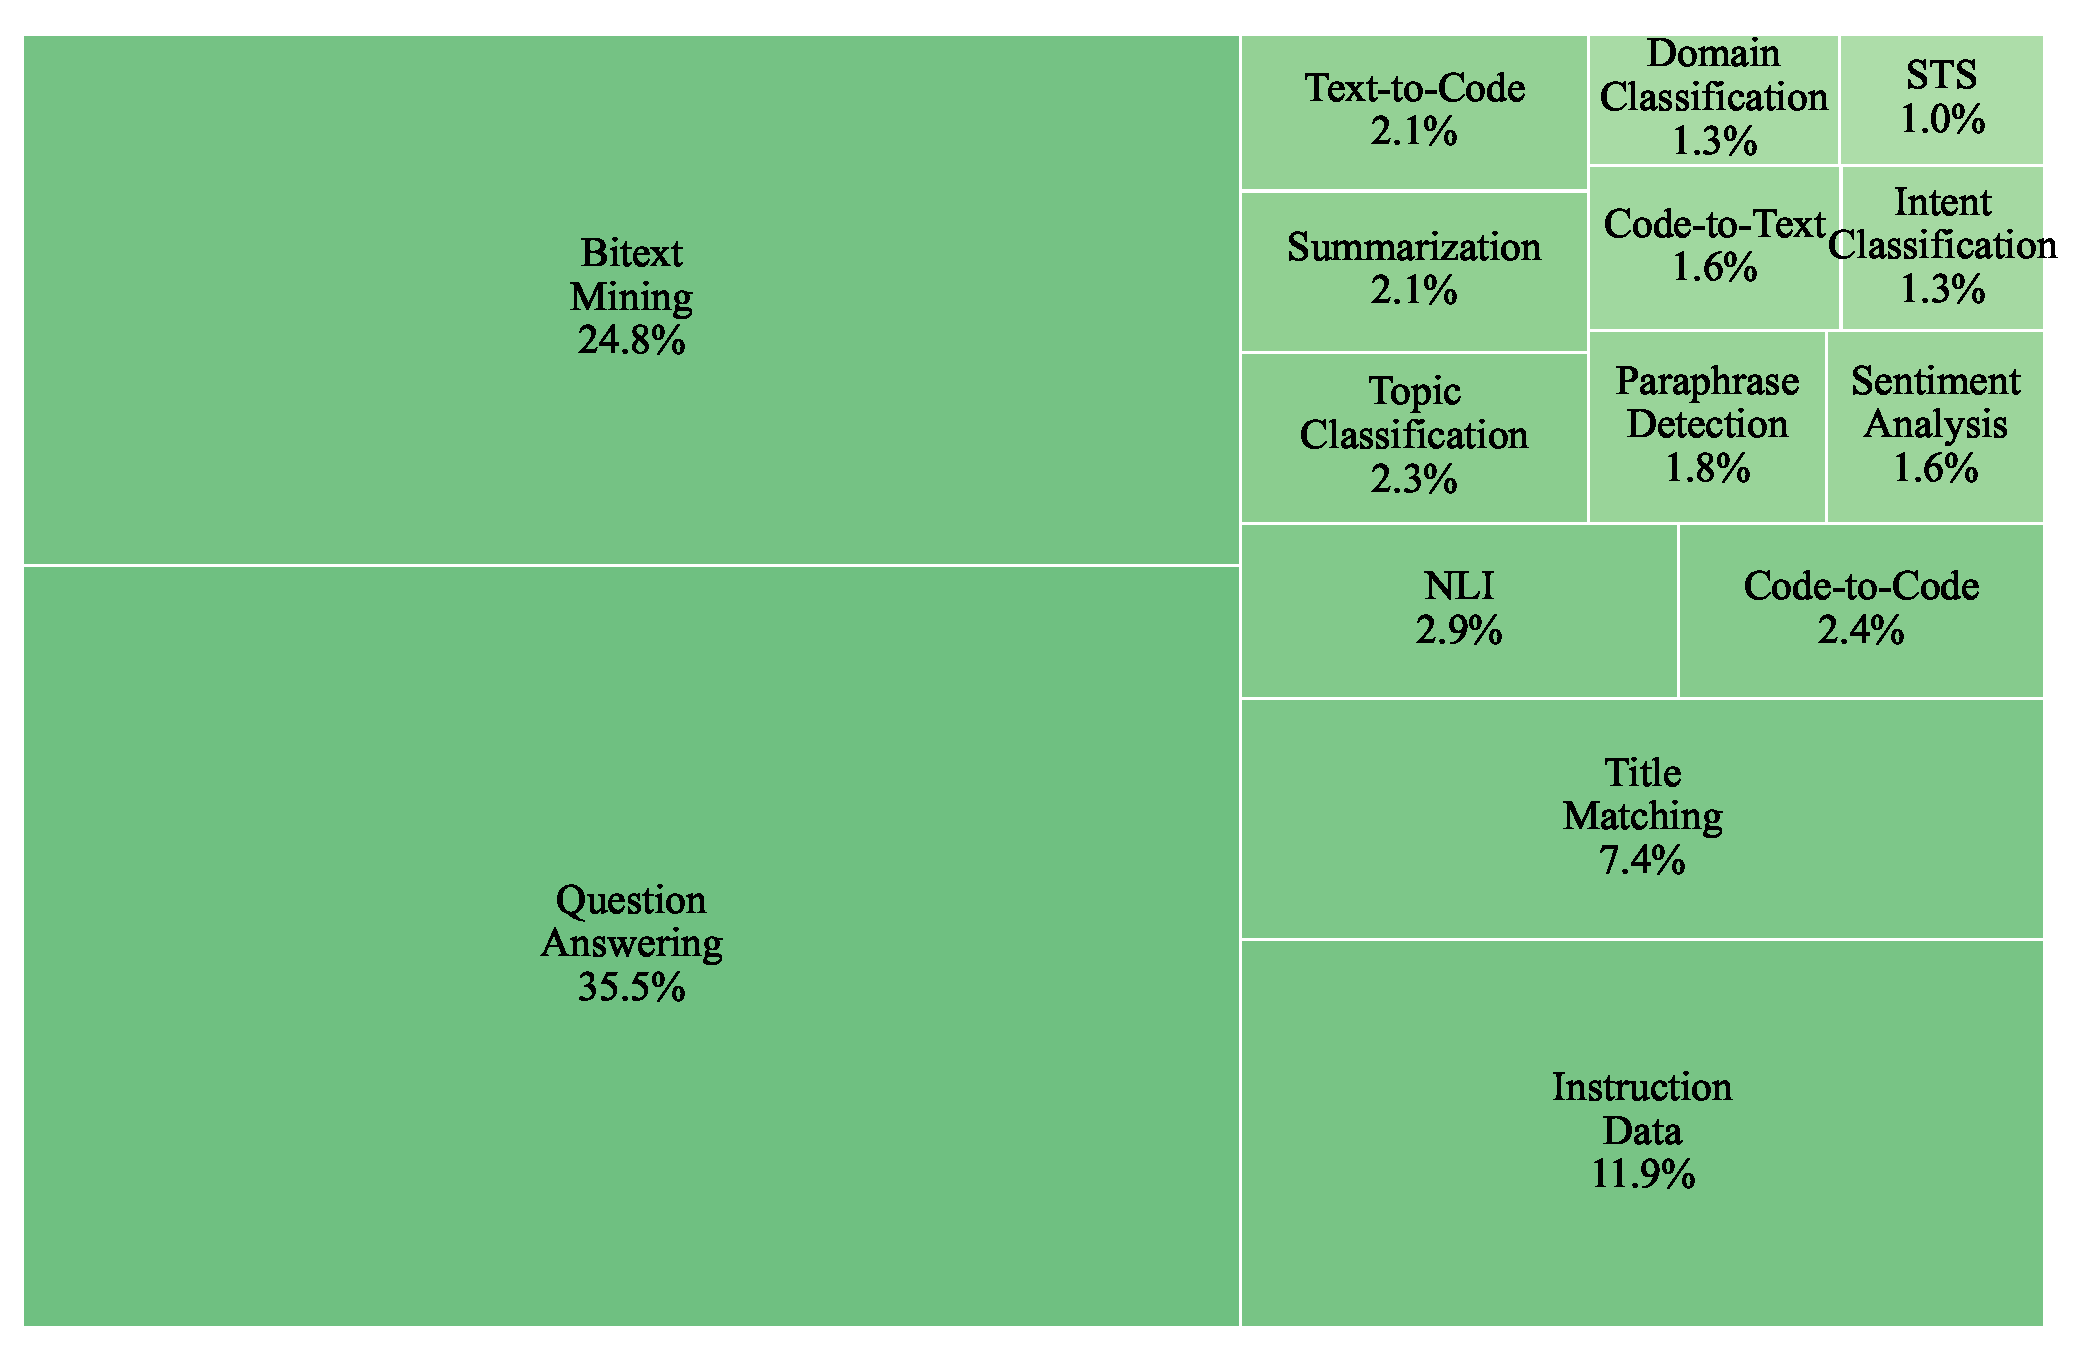
\includegraphics[width=0.7\linewidth]{figures/topic_distribution.pdf}
    \caption{Task type distribution in our training data.}
    \label{fig:task-distribution}
\end{figure}




The functional diversity of our dataset is equally critical for training a general-purpose embedding model. As shown in Figure~\ref{fig:task-distribution}, our collection encompasses a wide spectrum of tasks, ranging from retrieval-focused question answering and bitext mining to classification-oriented sentiment analysis and intent/domain classification.

To leverage this heterogeneity within a unified contrastive learning framework, we follow the first generation of F2LLM~\citep{2025f2llm} and consolidate all data into three canonical formats: \emph{retrieval, clustering, and two-way classification}. This consolidation allows the model to learn a versatile embedding space by optimizing a single, consistent objective across disparate data sources and task structures. For the retrieval format, data consists of (query, positive document, hard negatives) tuples. We leverage both in-batch negatives, where other documents in a mini-batch serve as negatives, and explicitly provided hard negatives (mined using Qwen3-Embedding-8B) to create a challenging and efficient training signal. For the clustering format, which also ingests multi-class classification tasks, tuples are formed by sampling an anchor, a positive example from the same class, and a hard negative from a different class. Finally, the two-way classification format directly uses class labels, where a given text serves as the anchor, the corresponding label text is the positive, and the opposite label text is the negative. For both clustering and classification, only hard negatives are utilized to avoid introducing false negatives from in-batch samples.

\begin{table}[]
    \small
    \centering
    \begin{tabular}{lrrrrrrrr}
    \toprule
        & \tb{80M} & \tb{160M} & \tb{330M} & \tb{0.6B} & \tb{1.7B} & \tb{4B} & \tb{8B} & \tb{14B} \\
    \midrule
        \rowcolor{gray!15} \multicolumn{9}{c}{\textit{Model Configuration}}\\
        Hidden Size & 320 & 640 & 896 & 1024 & 2048 & 2560 & 4096 & 5120 \\
        MLP Intermediate Size & 2048 & 1536 & 2560 & 3072 & 6144 & 9728 & 12288 & 17408 \\
        Transformer Layers & 8 & 9 & 16 & 28 & 28 & 36 & 36 & 40 \\
        Attention Heads & 16 & 16 & 16 & 16 & 16 & 32 & 32 & 40 \\
        KV Heads & 8 & 8 & 8 & 8 & 8 & 8 & 8 & 8 \\
        Head Dimension & 128 & 128 & 128 & 128 & 128 & 128 & 128 & 128 \\
    \midrule
        \rowcolor{gray!15} \multicolumn{9}{c}{\textit{Model Size}}\\
        Embedding Parameters & 49M & 97M & 136M & 156M & 311M & 389M & 622M & 778M \\
        Non-Embedding Parameters & 31M & 62M & 198M & 440M & 1409M & 3634M & 6946M & 13212M \\
        Total Parameters & 80M & 159M & 334M & 596M & 1721M & 4022M & 7568M & 13990M \\
    \midrule
        \rowcolor{gray!15} \multicolumn{9}{c}{\textit{Training Configuration}}\\
        MRL Support & $\surd$ & $\surd$ & $\surd$ & $\surd$ & $\surd$ & $\surd$ & $\surd$ & $\surd$ \\
        Learning Rate & 4e-5 & 3e-5 & 2e-5 & 1e-5 & 9e-6 & 7e-6 & 6e-6 & 5e-6 \\
        Epochs & 4 & 3 & 3 & 2 & 2 & 2 & 2 & 2 \\
        Batch Size & 512 & 512 & 512 & 512 & 512 & 512 & 512 & 512 \\
        Teacher & 0.6B & 0.6B & 0.6B & 1.7B & 4B & - & - & -\\
    \bottomrule
    \end{tabular}
    \caption{F2LLM-v2 model and training configurations.}
    \label{tab:model_config}
\end{table}

\subsection{Model Architecture}

We train models in 8 distinct sizes: 80M, 160M, 330M, 0.6B, 1.7B, 4B, 8B, and 14B. All models adopt a standard dense Transformer decoder architecture based on Qwen3~\citep{2025Qwen3}, and utilize the final hidden states of the EOS token as sequence representation. The detailed model configurations are given in Table~\ref{tab:model_config}. Models from 0.6B to 14B directly correspond to Qwen3 LLMs, while the 80M, 160M, and 330M models are pruned from the 0.6B model.

\subsection{Two-stage Training}\label{sec:method-training}

We adopt a two-stage training strategy following previous works~\citep{2025NV-Embed,2025Qwen3-Embedding}. The first stage focuses on building a robust semantic foundation, and 7 retrieval datasets are selected based on their large scale and broad language coverage, totalling 27 million samples: CodeSearchNet, CodeSearchNet-CCR, OpenCodeGeneticInstruct, WebFAQ, MMARCO, CLIRMatrix, and ParaCrawl (refer to Appendix~\ref{appendix:data} for details). Five models (0.6B-14B) are trained in this stage, and we employ the raw data without applying any instructional prefix.

The second stage aims to sharpen the model's ability to handle the nuances of diverse downstream applications like classification, reranking, and paraphrase detection. For this stage, we sample at most 80 thousand queries from each data source, producing a mixture of 18 million samples. We apply task-specific instructions to the queries, and also randomly apply instructions to 30\% of documents and negatives in tasks where queries and documents are symmetric, including clustering, STS, bitext mining, and paraphrase detection.

\paragraph{Pruning and Knowledge Distillation} After stage 1 training, we prune the 0.6B model to three smaller sizes along three dimensions: hidden size, MLP intermediate size, and number of layers. For hidden size and MLP intermediate size, we prune the rows and columns in associated weight matrices based on activation norms on a small set of calibration data. For the layer dimension, we simply keep the first $n$ layers of the model. We also experimented with pruning layers based on the change of activation norms, but found it to underperform this simple method.

After pruning, we find that naive training leads to large performance drops (see Table~\ref{tab:results-distillation}). We mitigate this by applying an additional knowledge distillation loss when training the pruned models, computed by the MSE between the student's sequence embedding and a teacher's sequence embedding over input query, document, and negatives. Ablation experiments suggest that this form of knowledge distillation can also benefit larger models, so we apply it to the 0.6B and 1.7B models in the second training stage as well, while the three largest models are trained without distillation due to resource constraints.

All models are trained with AdamW optimizer~\citep{2019AdamW}. Matryoshka Representation Learning~\citep{2022MRL} is applied in both training stages, with a minimum matryoshka dimension of 8. The remaining training hyperparameters are given in Table~\ref{tab:model_config}